

sminresでは,すべてのシフトに対して共通の基底を用いて反復計算を行う.  
この構造は,シフトごとの処理が独立であることから,\textbf{高い並列性}を有する.

本研究では,以下の2種類の並列化モデルを実装・比較した:

\vspace{10pt}
\textcolor{red}{モデル1}:ベクトル分割(MPI)+シフト分割(OpenMP)
\begin{itemize} \setlength{\itemsep}{0pt}
	\item MPI によるベクトルの\textcolor{red}{行方向分割}(ドメイン分割)
	\item OpenMP による各プロセス内でシフトループを並列化(M 個の方程式)
	\item 行列ベクトル積,内積,ノルム演算で通信を必要とする
\end{itemize}
\vspace{0.5em}
\textcolor{red}{モデル2}:シフト分割(MPI)+シフト分割(openMPI)
\begin{itemize} \setlength{\itemsep}{0pt}
	\item MPI によりプロセスに対してシフトを割り当て,完全に\textcolor{red}{独立なシフト分散}
	\item OpenMP により担当シフト内でループを並列化
	\item 通信を必要としない(行列は各プロセスが全体を保持)
\end{itemize}

\vspace{1.06pt}
\begin{figure}[H]
	\begin{center}
		\begin{minipage}[t]{0.49\columnwidth}
			\centering
			\colorbox{white}{ 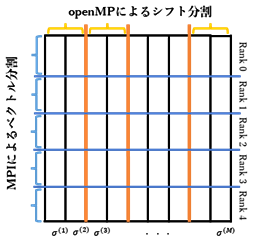
\includegraphics[scale=2.1]{./fig/parallel-model1.png} }
			\caption{並列化モデル1}
			\label{fig-parallel-model1}
		\end{minipage}
		\begin{minipage}[t]{0.49\columnwidth}
			\centering
			\colorbox{white}{ 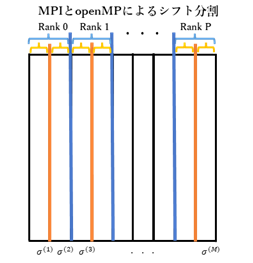
\includegraphics[scale=2.1]{./fig/parallel-model2.png} }
			\caption{並列化モデル2}
			\label{fig-parallel-model2}
		\end{minipage}
	\end{center}
\end{figure}

\vspace{5pt}
モデル1における通信の詳細:
\begin{table}[H]
	\centering
	\small
	\begin{tabular}{|c|l|l|c|}
	\hline
	行番号	& \multicolumn{1}{c|}{MPI関数}	& \multicolumn{1}{c|}{目的}				& 通信量	\\ \hline
	5		& \texttt{MPI\_Allgatherv}	& 部分ベクトルを集約し,全体ベクトルを構成		& $O(N)$	\\ \hline
	6		& \texttt{MPI\_Allreduce}	& 局所内積の合計を求め,全プロセスに共有		& $O(1)$	\\ \hline
	8		& \texttt{MPI\_Allreduce}	& 局所平方和の合計を求め,全プロセスに共有	& $O(1)$	\\ \hline
	\end{tabular}
\end{table}



\begin{comment}

\vspace{0.5em}
通信のうち最も支配的なのは毎反復ごとの \texttt{MPI\_Allgatherv} であり,
プロセス数が増えると通信待機時間がボトルネックとなりやすい.

そのため,モデル1はプロセス間通信のオーバーヘッドが問題となる場合に,
通信回数を抑える工夫やモデル2との併用が有効である.


通信の中でも特に \texttt{MPI\_Allgatherv} による全体ベクトルの共有は,
通信量・同期の両面でボトルネックとなりうる.

そのため,モデル1は通信待機時間の削減や非同期化技術との組み合わせが今後の課題となる.

\end{comment}